% select theme
\documentclass[t,8pt,aspectratio=169]{beamer}

% ====================================================
% ====================================================
% USEPACKAGES
% ====================================================
% ====================================================

\usepackage[T1]{fontenc}
\usepackage[utf8]{inputenc}
\usepackage[english]{babel}

% tables
\usepackage{tabularx}
\usepackage{colortbl}
\usepackage{multirow}
\usepackage{makecell}

% tikz and colors
\usepackage{tikz}
\usepackage{xcolor}
\usepackage{pgf-pie}
\usepackage{pgfplots}
\usepackage{pgfplotstable}
\usepackage{tikzsymbols}

\usetikzlibrary{calc}
\usetikzlibrary{trees}
\usetikzlibrary{patterns}
\usetikzlibrary{shadings}
\usetikzlibrary{positioning}
\usetikzlibrary{intersections}
\usetikzlibrary{decorations.pathreplacing}

\usetikzlibrary{arrows}
\usetikzlibrary{arrows.meta}

\usetikzlibrary{shapes}
\usetikzlibrary{shapes.arrows}
\usetikzlibrary{shapes.callouts}
\usetikzlibrary{shapes.symbols}
\usetikzlibrary{shapes.geometric}

\usepgfplotslibrary{patchplots}
\usepgfplotslibrary{fillbetween}

% boxes
\usepackage[many]{tcolorbox}

% math packages and fonts
\usepackage{bm}
\usepackage{ccfonts}
\usepackage{eulervm}
\usepackage{amsmath}
\usepackage{amsfonts}
\usepackage{amssymb}
\usepackage{amsthm}
\usepackage{mathtools}
\usepackage{nicefrac}
\usepackage{slashed}
\usepackage{bbold}
\usepackage{array}
\usepackage{cancel}

% algorithms and listings
\usepackage[ruled,vlined,linesnumbered]{algorithm2e}
\usepackage{listings}
\usepackage{setspace}

\tcbuselibrary{listings}
\tcbuselibrary{breakable}
\tcbuselibrary{skins}

% misc
\usepackage{soul}
\usepackage{pifont}
\usepackage{skull}
\usepackage{multicol}
\usepackage{animate}
\usepackage{cleveref}
\usepackage{hyperref}
\usepackage{wasysym}
\usepackage[absolute,overlay]{textpos}
\usepackage[hang,flushmargin]{footmisc}
\usepackage[framemethod=tikz]{mdframed} 				% provides frame for framed figure and framed table in theme_2

% ====================================================
% ====================================================
% COLOR DEFINITIONS
% ====================================================
% ====================================================

\definecolor{myblue1}{RGB}{35,119,189}
\definecolor{myblue2}{RGB}{95,179,238}
\definecolor{myblue3}{RGB}{129,168,207}
\definecolor{myblue4}{RGB}{26,89,142}

\definecolor{myred1}{RGB}{247,12,12}

% ====================================================
% ====================================================
% COMMON COMMANDS AND DEFINITIONS
% ====================================================
% ====================================================

% math definitions
% ====================================================
% argmin, argmax
\DeclareMathOperator*{\argmax}{arg\,max}
\DeclareMathOperator*{\argmin}{arg\,min}

% integration d
\newcommand*\diff{\mathop{}\!\mathrm{d}}

% independent sign
\newcommand{\indep}{\rotatebox[origin=c]{90}{$\models$}}

% vertical and horizontal bar
\newcommand*{\vertbar}{\rule[-1ex]{0.5pt}{2.5ex}}
\newcommand*{\horzbar}{\rule[.5ex]{2.5ex}{0.5pt}}

% math cancel sign
\newcommand\hcancel[2][black]{\setbox0=\hbox{$#2$}%
	\rlap{\raisebox{.45\ht0}{\textcolor{#1}{\rule{\wd0}{1pt}}}}#2}

% column type for matrices
\newcolumntype{C}[1]{>{\centering\arraybackslash}p{#1}}

% table definitions
% ====================================================
% centered X column in tabularx
\newcolumntype{Y}{>{\centering\arraybackslash}X}

% font commands
% ====================================================
% style of hyperlinks
\newcommand{\linkstyle}[1]{\underline{\smash{\texttt{#1}}}}

% slide architecture
% ====================================================
% divide frame into two parts
\newcommand{\divideTwo}[4]{
	\begin{minipage}{#1\textwidth}
		#2
	\end{minipage}
	\hfill
	\begin{minipage}{#3\textwidth}
		#4
	\end{minipage}
}

% divide frame into two parts (start on top)
\newcommand{\divideTwoTop}[4]{
	\begin{minipage}[t]{#1\textwidth}
		#2
	\end{minipage}
	\hfill
	\begin{minipage}[t]{#3\textwidth}
		#4
	\end{minipage}
}


% ====================================================
% ====================================================
% LAYOUT AND THEME
% ====================================================
% ====================================================

% adjust margin left and right
\setbeamersize{text margin left=25pt,text margin right=25pt}

% define colors
% ====================================================
\setbeamercolor{frametitle}{fg=black}
\setbeamercolor{itemize item}{fg=black}
\setbeamercolor{itemize subitem}{fg=black}
\setbeamercolor{caption name}{fg=black!80!white}
\setbeamercolor{section in toc}{fg=black}
\setbeamercolor{subsection in toc}{fg=gray!20!black}

% define fonts and sizes
% ====================================================
\setbeamerfont{frametitle}{series=\bf,size=\footnotesize}
\setbeamerfont{caption name}{series=\bf}
\setbeamertemplate{itemize/enumerate subbody begin}{\normalsize}
\setbeamertemplate{itemize/enumerate subsubbody begin}{\small}
\usefonttheme[onlymath]{serif}

% table of contents
% ====================================================
\makeatletter
\def\beamer@endinputifotherversion#1{}
\def\beamer@sectionintoc#1#2#3#4#5{{\large \vspace*{3mm} \textbf{#2} \hfill \textbf{#3} \par}}
\def\beamer@subsectionintoc#1#2#3#4#5#6{{\normalsize \hspace*{3mm} \textbf{#3} \hfill \textbf{#4} \par}}
\def\beamer@subsubsectionintoc#1#2#3#4#5#6#7{{\normalsize \hspace*{6mm} \textbf{#4} \hfill #5 \par}}
\makeatother

% define bullet points
% ====================================================
\setbeamertemplate{itemize item}[circle]
\setbeamertemplate{itemize subitem}{--}
\setbeamertemplate{itemize subsubitem}{\textcolor{black}{$\triangleright$}}
\setlength{\leftmargini}{3.5mm}
\setlength{\leftmarginii}{3.5mm}
\setlength{\leftmarginiii}{3.5mm}

% frametitle
% ====================================================
\setbeamertemplate{frametitle}{%
	\vspace*{1mm}
	\ifthenelse{\boolean{deeptoc}}{
		\ifnum\insertframenumber=\insertsectionstartpage%
			\vspace*{0.1mm}
    			\begin{tcolorbox}[
				skin=enhanced,
      				boxrule=0.6mm, boxsep=0mm,
     	   			lowerbox=ignored,
        			colback=orange!60!red, colframe=black,
        			borderline={0.5pt}{3pt}{black}, borderline={1pt}{2pt}{red}
    			]
        			\centering
        			\Huge\textbf\insertsectionhead\par
    			\end{tcolorbox}
		\fi%
	}{}
	\ifnum\insertframenumber=\insertsubsectionstartpage%
    		\vspace*{0.1mm}
    		\begin{tcolorbox}[
     		   	boxrule=0.4mm, boxsep=-0.5mm,
     	   		lowerbox=ignored,
     	   		colback=yellow!60!orange, colframe=black
    		]
        		\centering
        		\huge\textbf\insertsubsectionhead\par
   	 	\end{tcolorbox}
	\fi%
	\begin{tcolorbox}[
    		boxrule=0.2mm,
    		boxsep=0mm,
    		lowerbox=ignored,
    		colback=yellow, colframe=black
	]
    		\centering
    		\large\insertframetitle
	\end{tcolorbox}
	\vspace*{-2mm}
}

% header and Footer
% ====================================================

% header
\setbeamertemplate{headline}{
	% skip header line on first frame of section
	\ifnum\insertsectionstartframe=\insertframenumber%
     		\vskip-\headheight%
	\else
		\begin{beamercolorbox}[wd=\textwidth,ht=4mm,dp=1mm]{}
			\hspace*{25pt} \Fheadline \hspace{25pt}
		\end{beamercolorbox}
		\centerline{\rule{\linewidth}{.2pt}}
	\fi
}

\setbeamertemplate{footline}{%
	\centerline{\rule{\linewidth}{.2pt}}
	\begin{beamercolorbox}[wd=\textwidth,ht=2mm,dp=3mm]{}
		\hspace*{25pt} \Ffootline \hspace{25pt}
	\end{beamercolorbox}
}

% definition of header
\newcommand{\Fheadline}{
	\ifx\insertshorttitle\undefined
		\inserttitle
	\else
		\insertshorttitle
	\fi
	\hfill
	\insertsection
}

% definition of footer
\newcommand{\Ffootline}{
	\textbf{\insertauthor,~\insertinstitute,~\insertdate}
	\hfill
	\insertframenumber
}

% customize captions
% ====================================================
\setbeamertemplate{caption}{%
	\begin{tcolorbox}[
		colback=lightgray, colframe=black,
		width=.17\linewidth,
		height=17pt,
		boxrule=0.5pt, boxsep=-1pt
	]
		\textbf{\strut\insertcaptionname~\insertcaptionnumber%
		\usebeamertemplate{caption label separator}}%
	\end{tcolorbox}%
	\space%
	\begin{tcolorbox}[
		colback=lightgray, colframe=black,
		width=.82\linewidth,
		height=17pt,
		boxrule=0.5pt, boxsep=-1pt
	]
		\strut\insertcaption%
	\end{tcolorbox}%
}

% remove navigation symbols
\setbeamertemplate{navigation symbols}{}

% remove header line on first frame of section
% ====================================================
\makeatletter
\newcount\beamer@sectionstartframe
\beamer@sectionstartframe=1
\apptocmd{\beamer@section}{\addtocontents{nav}{\protect\headcommand{%
            \protect\beamer@sectionframes{\the\beamer@sectionstartframe}{\the\c@framenumber}}}
}{}{}
\apptocmd{\beamer@section}%
{\beamer@sectionstartframe=\c@framenumber\advance\beamer@sectionstartframe by1\relax}{}{}
\AtEndDocument{
	\immediate\write\@auxout{\string\@writefile{nav}%
        	{\noexpand\headcommand{\noexpand\beamer@sectionframes{\the\beamer@sectionstartframe}%
	{\the\c@framenumber}}}}
}{}{}

\def\beamer@startframeofsection{1}
\def\beamer@endframeofsection{1}
\def\beamer@sectionframes#1#2{%
    		\ifnum\c@framenumber<#1%
    		\else%
    			\ifnum\c@framenumber>#2%
    			\else%
    				\gdef\beamer@startframeofsection{#1}%
    				\gdef\beamer@endframeofsection{#2}%
    			\fi%
    		\fi%
}

\newcommand\insertsectionstartframe{\beamer@startframeofsection}
\newcommand\insertsectionendframe{\beamer@endframeofsection}
\makeatother

% ====================================================
% ====================================================
% COMMANDS AND GENERAL DEFINITIONS
% ====================================================
% ====================================================

% variable definitions
% ====================================================
% variable deeptoc (deep or flat table of contents)
\newcommand{\dwDeepToc}[1]{
	\newboolean{deeptoc}
	\setboolean{deeptoc}{#1}
}

% adjust font
% ====================================================
\renewcommand*{\familydefault}{\sfdefault}

% framed floatings
% ====================================================
\newmdenv[
	innerlinewidth=0.05pt,
	roundcorner=4pt,
	linecolor=black,
	innerleftmargin=6pt,
	innerrightmargin=6pt,
	innertopmargin=6pt,
	innerbottommargin=6pt
]{mybox}

\newmdenv[
	innerlinewidth=0.05pt,
	roundcorner=4pt,
	linecolor=black,
	innerleftmargin=0pt,
	innerrightmargin=0pt,
	innertopmargin=0pt,
	innerbottommargin=-1pt
]{mytablebox}

% framed figure
\newcommand{\dwFigure}[3]{
	\begin{figure}
		\begin{mybox}
			\centering #1
  		\end{mybox}
  		\vspace{-4mm}
  		\caption{#2}
  		\label{#3}
	\end{figure}
	\vspace{-3mm}
}

% framed table
\newcommand{\dwTable}[4]{
	\begin{table}
		\begin{mytablebox}
			\renewcommand{\arraystretch}{#4} #1
		\end{mytablebox}
		\vspace{-2.5mm}
		\caption{#2}
		\label{#3}
	\end{table}
}

% sections and subsections
% ====================================================
% section command
\newcommand{\dwSection}[1]{
	\ifthenelse{\boolean{deeptoc}}{
		\section{#1}
	}{
		\section{#1}
		\subsection*{#1}
	}
}

% subsection command
\newcommand{\dwSubsection}[1]{\subsection{#1}}

% header
% ====================================================
% green header
\newcommand{\dwHeader}[1]{%
	\begin{tcolorbox}[
		boxrule=0.2mm, boxsep=-1mm,
		lowerbox=ignored,
		colback=green, colframe=black,
		hbox
	]
		\textbf{#1}
	\end{tcolorbox}
}

% alert box / info box
% ====================================================
\newcommand{\dwAlertBox}[1]{
	\vspace*{2mm}\hspace*{0.25mm}
	\begin{minipage}[c]{0.05\textwidth}
		\begin{tikzpicture}[rotate=180, transform shape]\thicki\end{tikzpicture}
	\end{minipage}
	\hfill
	\begin{minipage}[c]{0.92\textwidth}
		\begin{mybox}
			\textcolor{red}{\textbf{#1}}
		\end{mybox}
	\end{minipage}
}

\newcommand{\dwInfoBox}[1]{
	\vspace*{2mm}\hspace*{0.25mm}
	\begin{minipage}[c]{0.05\textwidth}
		\begin{tikzpicture}\thicki\end{tikzpicture}
	\end{minipage}
	\hfill
	\begin{minipage}[c]{0.92\textwidth}
		\begin{mybox}
			\textcolor{blue}{\textbf{#1}}
		\end{mybox}
	\end{minipage}
}

\newcommand{\thicki}{
	\draw[thick,fill=lightgray] (4.2,0) -- (4.5,0.5) -- (4.8,0) -- (4.2,0) -- cycle;
	\fill (4.45,0.05) rectangle (4.55,0.25);
	\fill (4.50,0.34) circle (1.5pt);
}

% custom itemize environment
% ====================================================
\let\tempone\itemize
\let\temptwo\enditemize
\renewenvironment{itemize}{\vspace*{1.5mm}\tempone\addtolength{\itemsep}{0.5\baselineskip}}{\temptwo}
\let\tempthree\enumerate
\let\tempfour\endenumerate
\renewenvironment{enumerate}{\vspace*{1.5mm}\tempthree\addtolength{\itemsep}{0.5\baselineskip}}{\tempfour}

% frames
% ====================================================
\newenvironment{dwHeaderFrame}[1]{
	\subsubsection{#1}
	\begin{frame}{#1}
}{
	\end{frame}
}

% special pages
% ====================================================
% title page
\newcommand{\dwPrintTitle}{
	{\usebackgroundtemplate{%
		\tikz[overlay,remember picture] \node[opacity=0.9, at=(current page.center)] {
  			
\includegraphics[height=\paperheight,width=\paperwidth]{../03_img/processor_red.jpg}
		};
	}
	\begin{frame}[plain]
		\begin{center}
			\begin{tcolorbox}[
				skin=enhanced,
	      			boxrule=0.6mm, boxsep=0mm,
				lowerbox=ignored,
				colback=orange!60!red, colframe=black,
				borderline={0.5pt}{3pt}{black}, borderline={1pt}{2pt}{red},
				width=\textwidth
			]
				\centering
				\Huge\textbf{\inserttitle}
			\end{tcolorbox}
			\vspace*{1.4cm}
			\begin{tcolorbox}[width=0.5\textwidth]
				\centering
				\textbf{\insertauthor} \\[2mm]
				\insertinstitute \\[2mm]
				\insertdate
			\end{tcolorbox}
			
			\begin{textblock}{1}(1,13.5)
				
\includegraphics[scale=0.04]{../03_img/logo_dhbw}
			\end{textblock}
		\end{center}
	\end{frame}}
}

% table of contents
\newcommand{\dwPrintToc}[1]{
	{\makeatletter
   		\setbeamertemplate{headline}[default]
   		\def\beamer@entrycode{\vspace*{-\headheight}}
	\makeatother

	\begin{frame}[allowframebreaks]
		\begin{tcolorbox}[
			skin=enhanced,
      			boxrule=0.6mm, boxsep=0mm,
			lowerbox=ignored,
			colback=orange!60!red, colframe=black,
			borderline={0.5pt}{3pt}{black}, borderline={1pt}{2pt}{red},
			width=\textwidth
		]
			\centering
			\huge\textbf{Agenda for this Unit}
		\end{tcolorbox}
		\vspace{2mm}
		
		{\renewcommand{\baselinestretch}{1.4}
		\tableofcontents}
	\end{frame}}
}

% hyperlinks
% ====================================================
% redefine cref (add a hyperlink)
\let\chyperref\cref % save original command under a new name
\renewcommand{\cref}[1]{\hyperlink{#1}{\textcolor{blue}{$\Rightarrow$ \chyperref{#1}}}}

\newcommand{\externalurl}[2]{\href{#1}{\textcolor{blue}{$\Rightarrow$ #2}}}


% ====================================================
% ====================================================
% OPTIONS
% ====================================================
% ====================================================

% number of levels in toc
\dwDeepToc{false}

% ====================================================
% ====================================================
% PRESENTATION DATA
% ====================================================
% ====================================================

\title[Association Rule Learning]{***** Advanced Machine Learning ***** Association Rule Learning}
\author{M.\,Sc. Daniel Wehner}
\date{Summer term 2020}
\institute{SAP\,SE / DHBW Mannheim}

% ====================================================
% ====================================================
% BEGIN OF DOCUMENT
% ====================================================
% ====================================================

\begin{document}

% Title frame
%______________________________________________________________________
\dwPrintTitle

% Agenda
%______________________________________________________________________
\dwPrintToc

% Section: Introduction
%______________________________________________________________________
\dwSection{Introduction}

% What is Association Rule Mining?
\begin{dwHeaderFrame}{What is Association Rule Mining?}
	\begin{itemize}
		\item Association rule mining belongs to the category of unsupervised learning.
		\item Association rules describe frequent co-occurrences in the data (\textbf{not necessarily causality!})
		\item Examples:
		\begin{itemize}
			\item Market basket analysis (\textit{Which products are frequently bought together? E.\,g. Amazon})
			\item Course schedule planning (\textit{Which courses are often attended together?})
			\item Other use cases: Marketing promotions, inventory management, customer relationship management (CRM) 
		\end{itemize}
		\item The general form of a rule is given by:
		\begin{equation}
			\overbracket{\{a_1, a_2, \dots, a_n\}}^{\text{\textbf{Antecedent}}} 
			\rightarrow 
			\overbracket{\{b_1, b_2, \dots, b_m\}}^{\text{\textbf{Consequent}}}
		\end{equation}
		\item Example: $\{ bread, cheese \} \rightarrow \{ wine \}$
	\end{itemize}
\end{dwHeaderFrame}


\begin{frame}
	\dwFigure{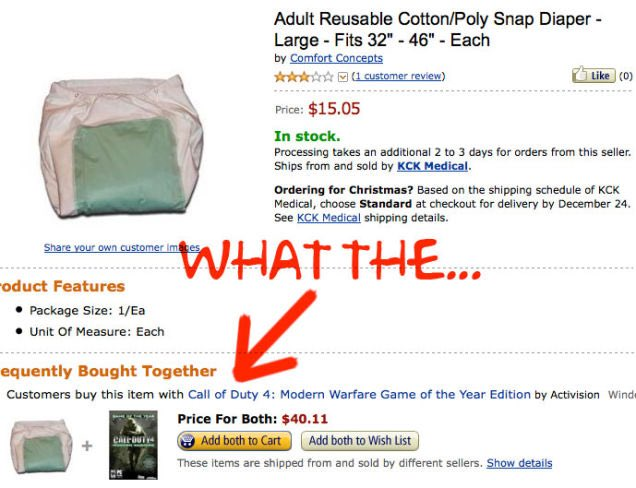
\includegraphics[scale=0.3]{16_association_rules/02_img/amazon}}{Famous example from Amazon}{fig:amazon}
\end{frame}


% Important Terminology
\begin{dwHeaderFrame}{Important Terminology}
	\begin{itemize}
		\item Suppose $\mathcal{I}$ is a set of unique items which we have in our portfolio,
			$\mathcal{T} = \{ t_1, t_2, \dots, t_n \}$ is a list of transactions (what customers bought).
		\item Each transaction $t_i \in \mathcal{T}$ is an element of $\mathfrak{P}(\mathcal{I})$, the power set of $\mathcal{I}$. (\textbf{What is a power set?})
		\item Example:
	\end{itemize}
	\dwFigure{
		\begin{minipage}{0.45\textwidth}
			\begin{table}[h]

\scalebox{0.8}{
	\begin{tabular}{| c | l |}
		\hline
		\textbf{Id} 		&
		\textbf{Transactions} 	\\ \hline\hline
		\textbf{1} 	& 	$\{ beer, chips, wine \}$ 		\\ \hline
		\textbf{2}	&	$\{ beer, chips \}$			\\ \hline
		\textbf{3}	&	$\{ pizza, wine \}$			\\ \hline
		\textbf{4}	&	$\{ chips, pizza \}$			\\ \hline
	\end{tabular}
}

\end{table}
		\end{minipage}
		\hfill
		\begin{minipage}{0.45\textwidth}
			\begin{table}[h]

\scalebox{0.8}{
	\begin{tabular}{| c | c | c | c | c |}
		\hline
		\textbf{Id} 	&
		$beer$	 	&
		$chips$		&
		$pizza$		&
		$wine$ 		\\ \hline\hline
		\textbf{1} & 1 & 1 & 0 & 1 \\ \hline
		\textbf{2} & 1 & 1 & 0 & 0 \\ \hline
		\textbf{3} & 0 & 0 & 1 & 1 \\ \hline
		\textbf{4} & 0 & 1 & 1 & 0 \\ \hline
	\end{tabular}
}

\end{table}
		\end{minipage}
	}{Left: List of transactions (raw), right: List of transactions in binary form}{}
	\dwInfoBox{Simplification: We ignore quantities and prices of the items sold.}
\end{dwHeaderFrame}


\begin{frame}
	\dwHeader{Item sets}
	\begin{itemize}
		\item A collection of $k$ items is called $k$-item set.
		\item Example: $\{ pizza, wine \}$ is a 2-item set.
		\item The number of items contained in a transaction $t_i$ is sometimes referred to as the \textbf{transaction width} $w(t_i) = \vert t_i \vert$.
		\item An important property of an item set $X$ is the \textbf{support count} $\bm{\sigma}$:
		\begin{equation}
			\sigma(X) = \vert \{ t_i \vert X \subseteq t_i \wedge t_i \in \mathcal{T} \} \vert
		\end{equation}
		\item \textbf{What does the support count tell us?} $\sigma(X)$ refers to the number of transactions $X$ occurs in.
	\end{itemize}
\end{frame}


% Quality Measures
\begin{dwHeaderFrame}{Quality Measures}
	\begin{itemize}
		\item \textit{Question:} How to measure the quality of an association rule?
		\item \textbf{Support:}
		\begin{itemize}
			\item Proportion of examples for which head and body are true.
			\item Example $A \rightarrow B$: How many customers bought $A$ and $B$ together?
			\begin{equation}
				\text{support}(A \rightarrow B) = \text{support}(A \cup B) = \frac{\sigma(A \cup B)}{n}
			\end{equation}
		\end{itemize}
		\item \textbf{Confidence:}
		\begin{itemize}
			\item Proportion of examples for which the head is true among those for which the body is true.
			\item Example: If customers bought $A$, how likely are they to also buy $B$?
			\begin{equation}
				\text{confidence}(A \rightarrow B) = \frac{\text{support}(A \cup B)}{\text{support}(A)} = \frac{\sigma(A \cup B)}{\sigma(A)}
			\end{equation}
		\end{itemize}
	\end{itemize}
\end{dwHeaderFrame}


\begin{frame}
	\begin{itemize}
		\item Support: There is a huge number of possible rules, but not all of them are interesting. \\
			$\Rightarrow$ \textbf{Prune (remove) rules with low support.}
		\item Confidence: The higher the confidence the more reliable is the rule.
		\item Example:
		\begin{itemize}
			\item $R = \{ bread, cheese \} \rightarrow \{ wine \}$
			\item $\text{support}(R) = 0.01$ and $\text{confidence}(R) = 0.8$
			\item 80\,\% of all customers who bought bread and cheese also bought red wine.
			\item However, only 1\,\% of the customers bought all three items together.
		\end{itemize}
	\end{itemize}
\end{frame}


% Section: Apriori
%______________________________________________________________________
\dwSection{Apriori}

% Learning Problem
\begin{dwHeaderFrame}{Learning Problem}
	\begin{itemize}
		\item The \textbf{Apriori algorithm} can be used to find association rules.
		\item The learning problem can be summarized as follows:
		\begin{quote}
			Given a set of transactions $\mathcal{T}$, find all rules having $\text{support} \ge s_{min}$ and $\text{confidence} \ge c_{min}$,
			where $s_{min}$ and $c_{min}$ are thresholds.
		\end{quote}
		\item Obviously, mining all possible rules is super expensive.
		\begin{equation}
			\vert \text{rules} \vert = 3^d - 2^{d+1} + 1 \qquad\text{where}\qquad d \equiv \vert \mathcal{I} \vert
		\end{equation}
		\item Also, rules can be spurious (i.\,e. patterns may occur by chance and are not systematic).
	\end{itemize}
	\dwAlertBox{We have to avoid considering all possible rules! $\Rightarrow$ Employ early pruning.}
\end{dwHeaderFrame}


% Early Pruning
\begin{dwHeaderFrame}{Early Pruning}
	\begin{itemize}
		\item The goal is to generate rules which have high support and high confidence.
		\item Observation: If an item set is infrequent (does not have sufficient support), calculating the confidence can be omitted.
		\item As a consequence, all rules which can be generated from this item set do not have to be considered anymore.
		\item Example for the item set $A = \{ beer, diapers, milk \}$:
		\begin{itemize}
			\item The rules derived from item set $A$ are given below.
			\item If we know item set $A$ to be infrequent, we can prune all these rules.
			\item There is no need to calculate the confidence for these rules (\textbf{decoupling of support and confidence}).
		\end{itemize}
	\end{itemize}
	\divideTwo{0.49}{
		\begin{align*}
			\{ beer, diapers \} 	&\rightarrow \{ milk \} 			\\
			\{ diapers, milk \}	&\rightarrow \{ beer \}		\\
			\{ milk \} 			&\rightarrow \{ beer, diapers \}	
		\end{align*}
	}{0.49}{
		\begin{align*}
			\{ beer, milk \} 		&\rightarrow \{ diapers \} 		\\
			\{ beer \}			&\rightarrow \{ diapers, milk \}	\\
			\{ diapers \}		&\rightarrow \{ beer, milk \}
		\end{align*}
	}
\end{dwHeaderFrame}


% Apriori Algorithm
\begin{dwHeaderFrame}{Apriori Algorithm}
	\begin{itemize}
		\item The overall algorithm consists of two major steps:
		\begin{enumerate}
			\item \textbf{Frequent item set generation:} \\
				Find all item sets which have sufficient support (satisfy the support constraint).
			\item \textbf{Rule generation:} \\
				Extract highly confident rules which satisfy the confidence constraint.
		\end{enumerate}
		\item In the following we will have a closer look at these two steps.
	\end{itemize}
\end{dwHeaderFrame}


\begin{frame}
	\dwHeader{Step 1) Frequent item set generation}
	\begin{itemize}
		\item It is possible to enumerate all possible item sets with a lattice \cref{fig:lattice}.
		\item A brute force approach could calculate the support for each candidate set and rank them by the result.
		\item \textbf{Problem:} The number of candidate sets grows exponentially with $\vert \mathcal{I} \vert$: $2^{\vert \mathcal{I} \vert} - 1$ (excluding empty set).
		\item Example: For $\mathcal{I} = \{ a, b, c, d, e \}$, we have 31 possible candidates.
		\item Therefore, the candidate sets should be generated more efficiently.
		\item We can make use of the \textbf{anti-monotonicity} of the support:
		\begin{quote}
			If an item set is frequent, then all of its subsets must be frequent as well. Also, if an item set is infrequent, then all its supersets must be infrequent too.
		\end{quote}
		\item Adding a condition can never increase the support of a rule:
		\begin{equation}
			A \subseteq B \Longrightarrow \text{support}(A) \ge \text{support}(B)
		\end{equation}
		\item \textbf{An item set can only be frequent, if all its subsets are frequent and all supersets of an infrequent item set are also infrequent.}
	\end{itemize}
\end{frame}


\begin{frame}
	\dwFigure{
		\begin{minipage}{0.30\textwidth}
			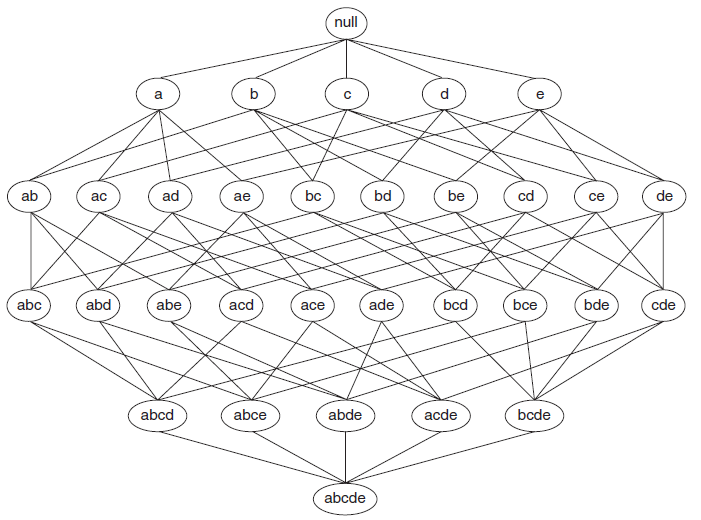
\includegraphics[scale=0.21]{16_association_rules/02_img/lattice1}
			\begin{center}(a) item set lattice\end{center}
		\end{minipage}
		\hfill
		\begin{minipage}{0.30\textwidth}
			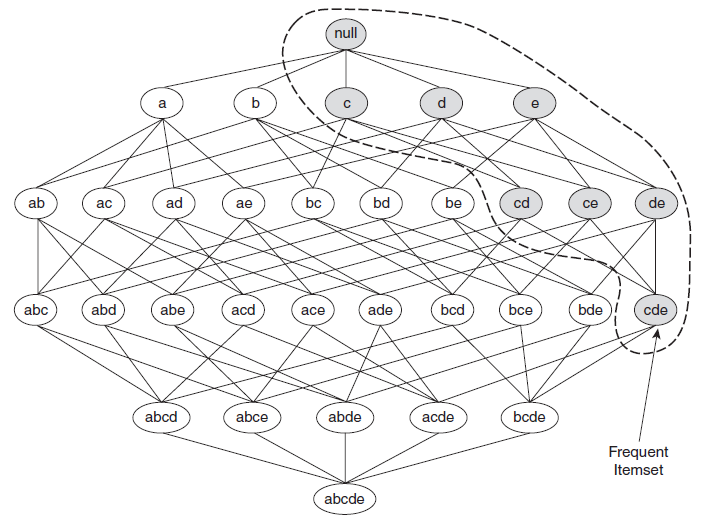
\includegraphics[scale=0.21]{16_association_rules/02_img/lattice2}
			\begin{center}(b) frequent item set\end{center}
		\end{minipage}
		\hfill
		\begin{minipage}{0.30\textwidth}
			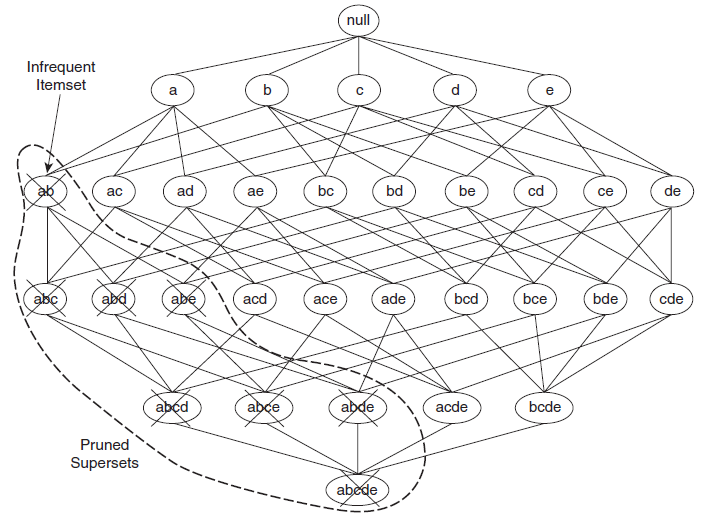
\includegraphics[scale=0.21]{16_association_rules/02_img/lattice3}
			\begin{center}(c) infrequent item set\end{center}
		\end{minipage}
	}{Item set lattice for $\mathcal{I} = \{ a, b, c, d, e \}$}{fig:lattice}
\end{frame}


\begin{frame}
	\begin{enumerate}
		\item $k \leftarrow 1$
		\item $C_1 \leftarrow \mathcal{I}$
		\item \textbf{while} $C_k \ne \emptyset$ \textbf{do}
		\begin{itemize}
			\item[$\triangleright$] $S_k \leftarrow C_k \backslash \{ \text{all infrequent item sets in $C_k$} \}$
			\item[$\triangleright$] $C_{k+1} \leftarrow \text{all sets with $k + 1$ elements which can be formed by uniting two item sets in $S_k$}$
			\item[$\triangleright$] $C_{k+1} \leftarrow C_{k+1} \backslash \{ \text{item sets, where not all subsets of size $k$ are in $S_k$} \}$
			\item[$\triangleright$] $S \leftarrow S \cup S_k$
			\item[$\triangleright$] $k \leftarrow k + 1$
		\end{itemize}
		\item \textbf{return} $S$
	\end{enumerate}

	\dwAlertBox{The algorithm leaves it open how the candidate set $C_{k+1}$ is generated. How can this be done efficiently?}
\end{frame}


\begin{frame}
	\begin{itemize}
		\item Requirements for efficient candidate generation:
		\begin{itemize}
			\item We have to avoid producing too many candidates.
			\item At the same time we have to ensure that all frequent item sets are found (\textbf{completeness})
			\item We don't want to produce duplicates (\textbf{efficiency})
		\end{itemize}
		\item The Apriori algorithm uses the following method:
		\begin{itemize}
			\item Merge a pair of $k$-item sets only if their first $k - 1$ items are identical.
			\begin{equation}
				A = \{ a_1, a_2, \dots, a_{k} \} \qquad\qquad\qquad B = \{ b_1, b_2, \dots, b_{k} \}
			\end{equation}
			\item Merge $A$ and $B$, if $a_j = b_j\ (j = 1, 2, \dots, k - 1) \wedge a_{k} \ne b_{k}$
			\item Example:
			\begin{itemize}
				\item $A = \{ bread, milk, pizza \}, B = \{ bread, milk, wine \}$
				\item $A$ and $B$ are merged into $\{ bread, milk, pizza, wine \}$.
			\end{itemize}
			\item This method still requires pruning non-frequent item sets.
			\item \textbf{Important: The item sets have to be in lexicographic order.}
		\end{itemize}
	\end{itemize}
\end{frame}


\begin{frame}
	Let's calculate the frequent item sets from the introductory example ($s_{min} = 0.25$):
	\begin{table}[h]

\scalebox{0.8}{
	\begin{tabular}{| c | c | c | c | c |}
		\hline
		\textbf{Id} 	&
		$beer$	 	&
		$chips$		&
		$pizza$		&
		$wine$ 		\\ \hline\hline
		\textbf{1} & 1 & 1 & 0 & 1 \\ \hline
		\textbf{2} & 1 & 1 & 0 & 0 \\ \hline
		\textbf{3} & 0 & 0 & 1 & 1 \\ \hline
		\textbf{4} & 0 & 1 & 1 & 0 \\ \hline
	\end{tabular}
}

\end{table}
	\begin{align*}
		C_1 	&= \{ \{ beer \}, \{ chips \}, \{ pizza \}, \{ wine \} \} \\
		S_1 	&= \{ \{ beer \}, \{ chips \}, \{ pizza \}, \{ wine \} \} \\
		C_2 	&= \{ \{ beer, chips \}, \{ beer, pizza \}, \{ beer, wine \}, \{ chips, pizza \}, \{ chips, wine \}, \{ pizza, wine \} \} \\
		S_2 	&= \{ \{ beer, chips \}, \{ beer, wine \}, \{ chips, pizza \}, \{ chips, wine \}, \{ pizza, wine \} \} \\
		C_3 	&= \{ \{ beer, chips, wine \}, \{ chips, pizza, wine \} \} \\
		S_3 	&= \{ \{ beer, chips, wine \} \} \\
		C_4 	&= \emptyset \\
		S 	&= \bigcup_{k=1}^3 S_k
	\end{align*}
\end{frame}


\begin{frame}
	\begin{itemize}
		\item The search space for frequent item sets can be structured using the subset relationship.
		\item \textbf{Border:}
		\begin{itemize}
			\item The border \cref{fig:border} consists of all item sets for which...
			\begin{itemize}
				\item ...all subsets are frequent and...
				\item ...no superset is frequent.
			\end{itemize}
			\item \textbf{Positive border:} Elements of the border which are frequent.
			\item \textbf{Negative border:} Elements of the border which are infrequent.
		\end{itemize}
	\end{itemize}
	
	\dwAlertBox{Frequent item sets = positive border plus all subsets of border elements}
\end{frame}


\begin{frame}
	\dwFigure{\begin{figure}
\centering
	\begin{tikzpicture}[
		scale=0.19,
		every node/.style={scale=0.75},
		box/.style={draw=black,very thick,minimum width=2.5cm,minimum height=0.5cm,align=center,fill=lightgray},
	]

		\draw[dashed,fill=lightgray!60,rounded corners=5pt] (-36,-20) -- (-24,-20) -- (-24,-13) -- (-12,-13) -- (-12,-20) -- (-14.25,-20) -- (-14.25,-27) -- (0.5,-27) -- (0.5,-20) -- (36,-20) -- (36,0) -- (-36,0) -- cycle;
		\node at (-30,-2) {frequent item sets};
		
		\node[box] (A) at (0,-2) {$\emptyset$};
		
		\node[box] (B) at (-21,-8) {$\{ beer \}$};
		\node[box] (C) at (-7,-8) {$\{ chips \}$};
		\node[box] (D) at (7,-8) {$\{ pizza \}$};
		\node[box] (E) at (21,-8) {$\{ wine \}$};
	
		\node[box] (F) at (-30,-16) {$\{ beer, chips \}$};
		\node[box] (G) at (-18,-16) {\textcolor{red}{$\bm{\{ beer, pizza \}}$}};
		\node[box] (H) at (-6,-16) {$ \{beer, wine \}$};
		\node[box] (I) at (6,-16) {\textcolor{green!40!black}{$\bm{\{ chips, pizza \}}$}};
		\node[box] (J) at (18,-16) {$\{ chips, wine \}$};
		\node[box] (K) at (30,-16) {\textcolor{green!40!black}{$\bm{\{ pizza, wine \}}$}};
	
		\node[box] (L) at (-21,-24) {$\{ beer, chips, pizza \}$};
		\node[box] (M) at (-7,-24) {\textcolor{green!40!black}{$\bm{\{ beer, chips, wine \}}$}};
		\node[box] (N) at (7,-24) {$\{ beer, pizza, wine \}$};
		\node[box] (O) at (21,-24) {\textcolor{red}{$\bm{\{ chips, pizza, wine \}}$}};
	
		\node[box] (P) at (0,-30) {$\{ beer, chips, pizza, wine \}$};
		
		\draw (A.south) -- (B.north);
		\draw (A.south) -- (C.north);
		\draw (A.south) -- (D.north);
		\draw (A.south) -- (E.north);
	
		\draw (B.south) -- (F.north);
		\draw (B.south) -- (G.north);
		\draw (B.south) -- (H.north);
		\draw (C.south) -- (F.north);
		\draw (C.south) -- (I.north);
		\draw (C.south) -- (J.north);
		\draw (D.south) -- (G.north);
		\draw (D.south) -- (I.north);
		\draw (D.south) -- (K.north);
		\draw (E.south) -- (H.north);
		\draw (E.south) -- (J.north);
		\draw (E.south) -- (K.north);
	
		\draw (F.south) -- (L.north);
		\draw (F.south) -- (M.north);
		\draw (G.south) -- (L.north);
		\draw (G.south) -- (N.north);
		\draw (H.south) -- (M.north);
		\draw (H.south) -- (N.north);
		\draw (I.south) -- (L.north);
		\draw (I.south) -- (O.north);
		\draw (J.south) -- (M.north);
		\draw (J.south) -- (O.north);
		\draw (K.south) -- (N.north);
		\draw (K.south) -- (O.north);
	
		\draw (L.south) -- (P.north);
		\draw (M.south) -- (P.north);
		\draw (N.south) -- (P.north);
		\draw (O.south) -- (P.north);
	
	\end{tikzpicture}
\end{figure}}{Border for the example above}{fig:border}
\end{frame}


\begin{frame}
	\dwHeader{Step 2) Generation of association rules}
	\begin{itemize}
		\item The frequent item sets can now be used to generate association rules.
		\item For each frequent $k$-item set $X$, there are $2^k - 2$ possible association rules (without $X \rightarrow \emptyset$ and $\emptyset \rightarrow X$) of the general form \cref{fig:rules}:
		\begin{equation}
			A \rightarrow B \qquad\text{with}\qquad A \cup B = X \wedge A \cap B = \emptyset 
		\end{equation}
		\item Calculate the confidence for the rules and check whether they fulfill the confidence constraint.
		\item We can also define \textbf{anti-monotonicity} for the confidence:
		\begin{quote}
			If a rule is not confident, moving conditions from body to head results in rules which are also not confident.
		\end{quote}
		\begin{equation}
			\text{confidence}(A \rightarrow B \cup C) \le \text{confidence}(A \cup B \rightarrow C)
		\end{equation}
		\item This circumstance can again be used for pruning the search space!
	\end{itemize}
\end{frame}


\begin{frame}
	\dwFigure{\begin{figure}
\centering
	\begin{tikzpicture}[
		scale=0.225,
		every node/.style={scale=0.8}
	]
		
		\node[align=center] (A) at (0,0) {$\{ beer, chips, wine \} \rightarrow \emptyset$ \\ \textcolor{red}{not a rule}};
	
		\node (B) at (-18,-6) {$\{ chips, wine \} \rightarrow \{ beer \}$};
		\node (C) at (0,-6) {$\{ beer, wine \} \rightarrow \{ chips \}$};
		\node (D) at (18,-6) {$\{ beer, chips \} \rightarrow \{ wine \}$};
	
		\node (E) at (-18,-12) {$\{ wine \} \rightarrow \{ beer, chips \}$};
		\node (F) at (0,-12) {$\{ chips \} \rightarrow \{ beer, wine \}$};
		\node (G) at (18,-12) {$\{ beer \} \rightarrow \{ chips, wine \}$};
	
		\node[align=center] (H) at (0,-18) {$\emptyset \rightarrow \{ beer, chips, wine \}$\\ \textcolor{red}{not a rule}};
	
		\draw[->] (A) -- (B);
		\draw[->] (A) -- (C);
		\draw[->] (A) -- (D);
	
		\draw[->] (B) -- (E);
		\draw[->] (B) -- (F);
		\draw[->] (C) -- (E);
		\draw[->] (C) -- (G);
		\draw[->] (D) -- (F);
		\draw[->] (D) -- (G);
	
		\draw[->] (E) -- (H);
		\draw[->] (F) -- (H);
		\draw[->] (G) -- (H);
	
	\end{tikzpicture}
\end{figure}}{Search space for association rules (frequent item set $\{ beer, chips, wine \}$)}{fig:rules}
\end{frame}


\begin{frame}
	Let's make a full example for the Apriori algorithm ($s_{min} = 0.5, c_{min} = 1.0$):
	\begin{table}[h]

\scalebox{0.8}{
	\begin{tabular}{| c | c | c | c | c | c |}
		\hline
		\textbf{Id}		&
		$bread$ 		&
		$butter$ 		&
		$coffee$ 		&
		$milk$		&
		$sugar$		\\ \hline\hline
		\textbf{1} & 1 & 1 & 0 & 0 & 1 \\ \hline
		\textbf{2} & 0 & 0 & 1 & 1 & 1 \\ \hline
		\textbf{3} & 1 & 0 & 1 & 1 & 1 \\ \hline
		\textbf{4} & 0 & 0 & 1 & 1 & 0 \\ \hline
	\end{tabular}
}

\end{table}
	\begin{align*}
		C_1 	&= \{ \{ bread \}, \{ butter \}, \{ coffee \}, \{ milk \}, \{ sugar \} \} \\
		S_1 	&= \{ \{ bread \}, \{ coffee \}, \{ milk \}, \{ sugar \} \} \\
		C_2 	&= \{ \{ bread, coffee \}, \{ bread, milk \}, \{ bread, sugar \}, \{ coffee, milk \}, \{ coffee, sugar \}, \{ milk, sugar \} \} \\
		S_2 	&= \{ \{ bread, sugar \}, \{ coffee, milk \}, \{ coffee, sugar \}, \{ milk, sugar \} \} \\
		C_3 	&= \{ \{ coffee, milk, sugar \} \} \\
		S_3 	&= \{ \{ coffee, milk, sugar \} \} \\
		C_4 	&= \emptyset \\
		S 	&= \bigcup_{k=1}^3 S_k
	\end{align*}
\end{frame}


\begin{frame}
	\begin{itemize}
		\item Rules with $c_{min} = 1.0$:
		\begin{tabbing}
			\hspace*{5cm}\=\hspace*{3cm}\=\kill
			$\{ bread \} \rightarrow \{ sugar \}$		\>	$s = 0.50$		\>	$c = 1.00$ 	\\[1.5mm]
			$\{ milk \} \rightarrow \{ coffee \}$		\>	$s = 0.75$		\>	$c = 1.00$ 	\\[1.5mm]
			$\{ coffee \} \rightarrow \{ milk \}$ 		\>	$s = 0.75$		\>	$c = 1.00$		\\[1.5mm]
			$\{ milk, sugar \} \rightarrow \{ coffee \}$	\>	$s = 0.50$		\>	$c = 1.00$		\\[1.5mm]
			$\{ coffee, sugar \} \rightarrow \{ milk \}$	\>	$s = 0.50$		\>	$c = 1.00$
		\end{tabbing}
		\item Other rules are either not frequent enough and are filtered out in step 1; \\
			e.\,g. $\{ butter \} \rightarrow \{ bread, sugar \}$, for which $s = 0.25$ and $c = 1.0$...
		\item ...or not confident enough and filtered out in step 2; \\
			e.\,g. $\{ milk, coffee \} \rightarrow \{ sugar \}$, for which $s = 0.5$ and $c = 0.67$.
	\end{itemize}
\end{frame}


% Section: Miscellaneous
%______________________________________________________________________
\dwSection{Miscellaneous}

% Interestingness
\begin{dwHeaderFrame}{Interestingness}
	\begin{itemize}
		\item \textbf{Problem:} There might still be way too many rules.
		\item Assume the following two rules:
		\begin{equation}
			R_1 =  A \cup B \rightarrow C \qquad\qquad\qquad R_2 = A \rightarrow C
		\end{equation}
		\item Filter out $R_1$, if the rule is...
		\begin{itemize}
			\item ...\textit{trivial} ($R_2$ covers the same examples)
			\item ...\textit{unproductive} ($R_2$ has equal or higher confidence)
			\item ...\textit{insignificant} (Confidence of $R_2$ is not significantly worse)
		\end{itemize}
		\item Filter by \textbf{interestingness} (\textit{How can we measure interestingness?})
	\end{itemize}
\end{dwHeaderFrame}


\begin{frame}
	\begin{itemize}
		\item Support and confidence are not sufficient to capture whether a rule is interesting or not.
		\item A rule may have high support and confidence, but still may not be interesting.
		\item Example:
		\begin{itemize}
			\item Consider the rule: $\{ diapers \} \rightarrow \{ beer \}; c = 0.90$
			\item 90\,\% of all customers who buy diapers also buy beer.
			\item Sounds like and interesting association rule.
			\item \textbf{But:} If we know, that 90\,\% of all customers buy beer, this rule is not interesting anymore.
		\end{itemize}
	\end{itemize}
\end{frame}


% Lift, Leverage and Conviction
\begin{dwHeaderFrame}{Lift, Leverage and Conviction}
	\begin{itemize}
		\item Consider rule $R = A \rightarrow B$
		\item \textbf{Lift:} Rule $R$ is interesting, if $\text{lift}(R) \gg 1$.
		\begin{equation}
			\text{lift}(A \rightarrow B) = \frac{\text{support}(A \rightarrow B)}{\text{support}(A) \cdot \text{support}(B)}
		\end{equation}
		\item \textbf{Leverage:} Rule $R$ is interesting, if $\text{leverage}(R) \gg 0$.
		\begin{equation}
			\text{leverage}(A \rightarrow B) = \text{support}(A \rightarrow B) - \text{support}(A) \cdot \text{support}(B)
		\end{equation}
		\item \textbf{Conviction:} Expected ratio that $A$ occurs without $B$ (incorrect prediction of $R$).
		\begin{equation}
			\text{conviction}(A \rightarrow B) = \frac{1 - \text{support}(B)}{1 - \text{confidence}(A \rightarrow B)}
		\end{equation}
	\end{itemize}
\end{dwHeaderFrame}

\end{document}
